% Chapter 2
\chapter{Digital Signal Process} % Main chapter title

\label{Chapter2} % For referencing the chapter elsewhere, use \ref{Chapter1}

\lhead{Chapter 2. \emph{Digital Signal Process}} % This is for the header on each page - perhaps a shortened title

\cite{wiki-dsp-sampling}
Sampling is the process of recording the values of a signal at given points in time. For A/D converters, these points in time are equidistant. The number of samples taken during one second is called the sample rate. Keep in mind that these samples are still analogue values. The mathematic description of the ideal sampling is the multiplication of the signal with a sequence of dirac pulses. In real A/D converters the sampling is carried out by a sample-and-hold buffer. The sample-and-hold buffer splits the sample period in a sample time and a hold time. In case of a voltage being sampled, a capacitor is switched to the input line during the sample time. During the hold time it is detached from the line and keeps its voltage.

\begin{figure}[ht]
  \label{fig:chap2-Analog_Waveform}
  \centering
	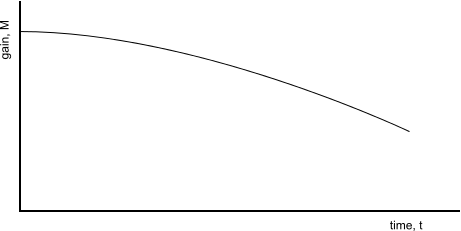
\includegraphics[width=0.7\textwidth, keepaspectratio=true]{chap2-Analog_Waveform.png}
	\caption{.}
\end{figure}
\begin{figure}[ht]
  \label{fig:chap2-Sampled_Waveform}
  \centering
	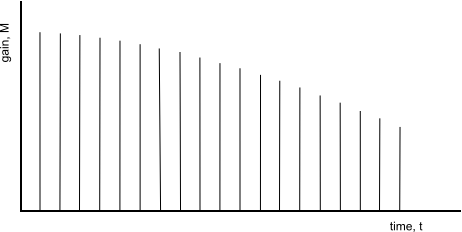
\includegraphics[width=0.7\textwidth, keepaspectratio=true]{chap2-Sampled_Waveform.png}
	\caption{.}
\end{figure}

\section{ADC and DAC}\cite{smith1997dspbook}
Most of the signals directly encountered in science and engineering are continuous: light intensity that changes with distance; voltage that varies over time; etc. Analog-to-Digital Conversion (ADC) and Digital-to-Analog Conversion (DAC) are the processes that allow digital computers to interact with these everyday signals. Digital information is different from its continuous counterpart in two important respects: it is sampled, and it is quantized. Both of these restrict how much information a digital signal can
contain. This chapter describes the sampling frequency, number of bits, and type of analog filtering needed for converting between the analog and digital.

\begin{compactitem}
\item \textbf{Quantization}
Quantization is the process of representing the analog voltage from the sample-and-hold circuit by a fixed number of bits. The input analog voltage (or current) is compared to a set of pre-defined voltage (or current) levels. Each of the levels is represented by a unique binary number, and the binary number that corresponds to the level that is closest to the analog voltage is chosen to represent that sample. This process rounds the analog voltage to the nearest level, which means that the digital representation is an approximation to the analog voltage. There are a few methods for quantizing samples. The most commonly used ones are the dual slope method and the successive approximation.

\begin{figure}[ht]
  \label{fig:chap2-Digital_Waveform}
  \centering
	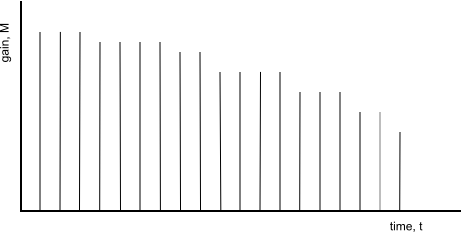
\includegraphics[width=0.7\textwidth, keepaspectratio=true]{chap2-Digital_Waveform.png}
	\caption{.}
\end{figure}


\item \textbf{The Sampling Theorem}\cite{dsp-nyquist}\\
The sampling theorem states that for a limited bandwidth (band-limited) signal with maximum frequency $f_{max}$, the equally spaced sampling frequency $f_s$ must be greater than twice of the maximum frequency $f_{max}$, i.e.,
$f_s > 2·f_{max}$
in order to have the signal be uniquely reconstructed without aliasing.

The frequency $2·f_{max}$ is called the \textbf{Nyquist sampling rate}. Half of this value, $f_{max}$, is sometimes called the \textbf{Nyquist frequency}.

\end{compactitem}

\section{Fourier Transform} \cite{csulb-Woollett}

\begin{compactitem}

\item {Fourier Series Expansion of a Function over $(-\boldsymbol{\pi,\,\pi})$}\\
A Fourier series expansion designed to represent a given function
  \textbf{f(x)} defined over a finite interval $(-\boldsymbol{\pi, \pi})$, is a sum of terms
\begin{equation}  \label{fxpi}
\mathbf{f(x) = \frac{1}{2} \, a_{0} + \sum_{n=1}^{\infty} \left[
   a_{n}\,\boldsymbol{\cos} (n\,x) + b_{n} \,\boldsymbol{\sin} (n\,x) \right] }
\end{equation}

\noindent and the constant coefficients ($\mathbf{a_{n},\, b_{n}}$) are
\begin{equation} \label{fcoeff}
 \mathbf{ a_{n} = \frac{1}{\boldsymbol{\pi}} \, \int_{-\boldsymbol{\pi}}^{\boldsymbol{\pi}} f(y)\,
   \boldsymbol{\cos} (n\,y) \, dy}, \quad
   \mathbf{ b_{n} = \frac{1}{\boldsymbol{\pi}} \, \int_{-\boldsymbol{\pi}}^{\boldsymbol{\pi}} f(y)\,
   \boldsymbol{\sin} (n\,y) \, dy}.
\end{equation}
(For a derivation of these equations see Sec.\ref{expfs} and Eqs.(\ref{Eq:piex1}) and
  (\ref{Eq:piex2}).)\\

\noindent The first term of the expansion
\begin{equation}
\mathbf{ \frac{1}{2} \, a_0  =
 \frac{1}{2\, \boldsymbol{\pi}}  \int_{-\boldsymbol{\pi}}^{\boldsymbol{\pi}} f(y)\,dy =
 \langle f(x) \rangle }
\end{equation}
is the (un-weighted) average of \textbf{f(x)} over the domain $(-\boldsymbol{\pi},\boldsymbol{\pi})$.
Hence $\mathbf{a_{0}}$ will always be twice the average value of the function over
  the domain.\\

\noindent If \textbf{f(x)} is an even function ($\mathbf{f(-x) =  f(x)}$),
  then only the $\mathbf{\boldsymbol{\cos}(n\,x)}$ terms
  contribute.
If \textbf{f(x)} is an odd function ($\mathbf{f(-x) =  -f(x)}$),
  then only the $\mathbf{\boldsymbol{\sin}(n\,x)}$ terms contribute. \\


\item {Fourier Transform}\\
\textbf{Fourier Cosine Integrals}
Given some function $\mathbf{f(x)}$ defined for $\mathbf{x \geq 0}$,
  we define the Fourier cosine transform  of this function as
\begin{equation}  \label{Eq:fc1}
\mathbf{F_{C}(f,\boldsymbol{\omega}) = \frac{2}{\boldsymbol{\pi}}
  \int_{0}^{\infty} \boldsymbol{\cos}(\boldsymbol{\omega}\,x)\,f(x)\,dx }
\end{equation}
The given function $\mathbf{f(x)}$ can then be written as an integral
  over positive values of $\boldsymbol{\omega}$:
\begin{equation}  \label{Eq:fc2}
\mathbf{f(x) = \int_{0}^{\infty} F_{C}(f,\boldsymbol{\omega})\,
    \cos(\boldsymbol{\omega}\,x)\,d\boldsymbol{\omega} }
\end{equation}
The two equations (\ref{Eq:fc1}) and (\ref{Eq:fc2}) are an example of
  a "Fourier transform pair", which include conventions about where
  to place the factor of $2/\boldsymbol{\pi}$.\\

\textbf{Fourier Sine Integrals}\\
Given some function $\mathbf{f(x)}$ defined for $\mathbf{x \geq 0}$,
  we define the Fourier sine transform  of this function as
\begin{equation}  \label{Eq:fsine1}
\mathbf{F_{S}(f,\boldsymbol{\omega}) = \frac{2}{\boldsymbol{\pi}}
  \int_{0}^{\infty} \boldsymbol{\sin}(\boldsymbol{\omega}\,x)\,f(x)\,dx }
\end{equation}
The given function $\mathbf{f(x)}$ can then be written as an integral
  over positive values of $\boldsymbol{\omega}$:
\begin{equation}  \label{Eq:fsine2}
\mathbf{f(x) = \int_{0}^{\infty} F_{S}(f,\boldsymbol{\omega})\,
    \sin(\boldsymbol{\omega}\,x)\,d\boldsymbol{\omega} }
\end{equation}
The two equations (\ref{Eq:fsine1}) and (\ref{Eq:fsine2}) are another
   "Fourier transform pair", which include conventions about where
  to place the factor of $2/\boldsymbol{\pi}$.

\textbf{Exponential Fourier Integrals}\\
Given some function $\mathbf{f(x)}$ defined for $\mathbf{-\infty <x < \infty}$,
  we define the exponential Fourier transform  of this function as
\begin{equation}  \label{Eq:fexp1}
\mathbf{F_{Exp}(f,\boldsymbol{\omega}) = \frac{1}{2\, \boldsymbol{\pi}}
  \int_{-\infty}^{\infty} \,f(x) e^{i\,\boldsymbol{\omega}\,x}\,dx }
\end{equation}
The given function $\mathbf{f(x)}$ can then be written as an integral
  over both positive and negative values of $\boldsymbol{\omega}$:
\begin{equation}  \label{Eq:fexp2}
\mathbf{f(x) = \int_{-\infty}^{\infty} F_{Exp}(f,\boldsymbol{\omega})\,
    e^{-i\,\boldsymbol{\omega}\,x} \,d\boldsymbol{\omega} }
\end{equation}
The two equations (\ref{Eq:fexp1}) and (\ref{Eq:fexp2}) are another
   "Fourier transform pair", which include conventions about where
  to place the factor of $\mathbf{2\, \boldsymbol{\pi}}$ as well as which member
  has the minus sign in the exponent.\\

\noindent If the given function is even, $\mathbf{f(-x) = f(x) }$, then the
exponential Fourier transform has the symmetry
\begin{equation}
\mathbf{F_{Exp}(f,\boldsymbol{-\omega}) = F_{Exp}(f,\boldsymbol{\omega}) }
\end{equation}
and can be expressed in terms of the Fourier cosine transform:
\begin{equation}
\mathbf{F_{Exp}(f,\boldsymbol{\omega}) = \frac{1}{2} \, F_{C}(f,\boldsymbol{\omega})}.
\end{equation}
If the given function is odd, $\mathbf{f(-x) = -f(x) }$, then the
exponential Fourier transform has the symmetry
\begin{equation}
\mathbf{F_{Exp}(f,\boldsymbol{-\omega}) = -F_{Exp}(f,\boldsymbol{\omega}) }
\end{equation}
and can be expressed in terms of the Fourier sine transform:
\begin{equation}
\mathbf{F_{Exp}(f,\boldsymbol{\omega}) = \frac{i}{2} \, F_{S}(f,\boldsymbol{\omega})}.
\end{equation}
If the given function is neither even nor odd, the function can always be written
  as the sum of an even function $\mathbf{f_{e}(x)}$ and an odd function $\mathbf{f_{o}(x)}$:
\begin{equation}
\mathbf{f(x) \equiv f_{e}(x) + f_{o}(x) =
  \frac{1}{2} \,( f(x) + f(-x) + \frac{1}{2} \, ( f(x) - f(-x) }
\end{equation}
and can be expressed in terms of the Fourier cosine transform of $\mathbf{f_{e}(x)}$
  and the Fourier sine transform of $\mathbf{f_{o}(x)}$:
\begin{equation}
\mathbf{F_{Exp}(f,\boldsymbol{\omega}) \equiv F_{Exp}(f_{e}+f_{o},\boldsymbol{\omega}) =
  \frac{1}{2} \, F_{C}(f_{e},\boldsymbol{\omega}) +
  \frac{i}{2} \, F_{S}(f_{o},\boldsymbol{\omega}) }
\end{equation}


\item {Discrete Fourier Transform}

\item {Fast Fourier Transform}

\item {Power Spectra}

\end{compactitem}

%----------------------------------------------------------------------------------------

\section{ICA}

You have reached the end of this mini-guide. You can now rename or overwrite this pdf file and begin writing your own `\texttt{Chapter1.tex}' and the rest of your thesis. The easy work of setting up the structure and framework has been taken care of for you. It's now your job to fill it out!

Good luck and have lots of fun!

\begin{flushright}
Guide written by ---\\
Sunil Patel: \href{http://www.sunilpatel.co.uk}{www.sunilpatel.co.uk}
\end{flushright}
